\documentclass[11pt,a4paper]{scrartcl}
\usepackage[utf8x]{inputenc}
\usepackage{ucs}
\usepackage{amsmath}
\usepackage{amsfonts}
\usepackage{amssymb}
\usepackage{graphicx}
\usepackage{fancyhdr}
\usepackage{gauss}
\usepackage{listings}
\usepackage{tabularx}
\usepackage[german, ruled, vlined]{algorithm2e}

\pagestyle{fancy}

\DeclareMathOperator*{\xor}{xor}%

\author{\textbf{Alexander Weigl} \and Timmie Yuen \and Daniel Wahlscheid}
\title{Übungen - Angewandte Kryptologie}

\newcommand{\qed}{\hfill \textbf{\#} }
\newcommand{\imp}{\Rightarrow}
\newcommand{\gdw}{\Leftrightarrow}
\renewcommand{\thesubsubsection}{\alph{subsubsection}}

\newcommand{\INT}{\mathbb{Z}}

\fancyhead[L]{\small{\today}}

%\includeonly{chapters/05}

\begin{document}

\maketitle
\tableofcontents
\newpage


\section{Übung 1}

\subsection{Aufgabe 1}

\begin{center}
\begin{tabular}{lcccr}
\textbf{Chiffre} & \textbf{Alphabet} & \textbf{Geheimtext} & \textbf{Schlüsselraum} & \textbf{Länge}                                  \\   \hline
Caesar  & $\{A, \cdots, Z \}$ & $\{A, \cdots, Z \}$ & $\{3\}, \{1, \cdots, 25 \}$ & 4,64     \\   \hline
OTP  	& $\{0,1 \}$  		  & $\{0,1 \}$      	& $\{0,1\}^*$ 				  & $\infty$ \\   \hline
DES  	& $\{0,1 \}$   		  & $\{0,1 \}$ 			& $\{0,1\}^{56}$ 		      & 56       \\   \hline
\end{tabular}
\end{center}
\subsection{Aufgabe 2}
\subsubsection{Beweis: Äquivalenzrelation: $\equiv_n$  }
\paragraph{Reflexivität}
\hspace{1cm} $ \forall x: x \equiv_n x $

\begin{equation}
	x \mod n \equiv r = x \mod n \imp x \equiv_{n} x 
\end{equation}
\qed

\paragraph{Symmetrie}
\hspace{1cm} $ \forall x,y: x \equiv_n y \imp y \equiv_n x $

\begin{align*}
	x \equiv_n y \mod n        
	& \imp 	x \mod n = r = y \mod n      \\ 
	& \imp	y \mod n = x \mod n        \imp  y \equiv_n x
\end{align*}
\qed


\paragraph{Transitiviät}
\hspace{1cm} $ \forall x,y,z: x \equiv_n y , y \equiv_n z => x \equiv_n z $

\begin{align*}
	n. V. & x \mod n = r_x,  										 \\
          & y \mod n = r_y  			   					     		 \\
          & z \mod n = r_z 										
           \wedge r_x = r_y , r_y=r_z \imp                           \\
		  & r_x = r_z \imp x \equiv_n z \mod n
\end{align*}
\qed

\subsubsection{}
\paragraph{} 
\hspace{1cm} \textbf{z.~Z.} $ [i]_n + [j]_n = [i+j]_n$

\begin{align*}
\text{Sei } a,b \in \INT &\imp a = q_an+r_a , b = q_bn+r_b    			 \\ \\
				 &\imp  a \in [r_a]_n , b \in  [r_b]_n  			     \\
				 &\imp [r_a]_n + [r_b]_n = \{ \forall i: in(r_a+r_b) \}	 \\
				 &\imp a + b =  q_an+r_a + q_bn+r_b                      \\
				 & \equiv_n   n(q_a+q_b)+r_a+r_b                   \\
				 & \equiv_n r_a+r_b  \imp [r_a+r_b]_n
\end{align*}

\paragraph{} 
\hspace{1cm} \textbf{z.~Z.} $ [i]_n \cdot [j]_n = [i \cdot j]_n$
\begin{align*}
\text{Sei } a,b \in \INT & \imp a = q_an+r_a , b = q_bn+r_b    			 \\ \\
				 &\imp  a \in [r_a]_n , b \in  [r_b]_n  			     \\
				 &\imp [r_a]_n * [r_b]_n = \{ \forall i: in(r_a*r_b) \}	 \\
				 &\imp a * b \equiv_n  (q_an+r_a) * (q_bn+r_b)                  \\
				 & \equiv_n  q_aq_bn+q_anr_b+q_bnr_a+r_a*r_b                   \\
				 & \equiv_n  n(q_aq_b+q_ar_b+q_br_a)+r_a*r_b                   \\				 
				 & \equiv_n r_a*r_b  =  [r_a+r_b]_n
\end{align*}

\subsection{}
\subsubsection{}
\begin{align*}
 ( 23.145 \cdot = 12.479 + 14.543 ) \cdot \mod 9 & \equiv_9 \\
 ( 6 \cdot 5 + 8 ) \cdot 5 & \equiv_9  3				    \\
 8 \cdot 5 &\equiv_9 \\
 2\cdot 5 \equiv_9 10 &= 1 \mod 9 
\end{align*}

\subsubsection{}
\begin{align*}
 123 \cdot  (123.983 \cdot 789.345 + 676.345) mod 11 & \equiv_{11} \\
 2    \cdot  (2 \cdot 7 + 10) & \equiv_{11}   \\
 2 \cdot (14 + 10 ) & \equiv_{11}  4 \mod 11
\end{align*}


\subsection{}

\begin{center}
	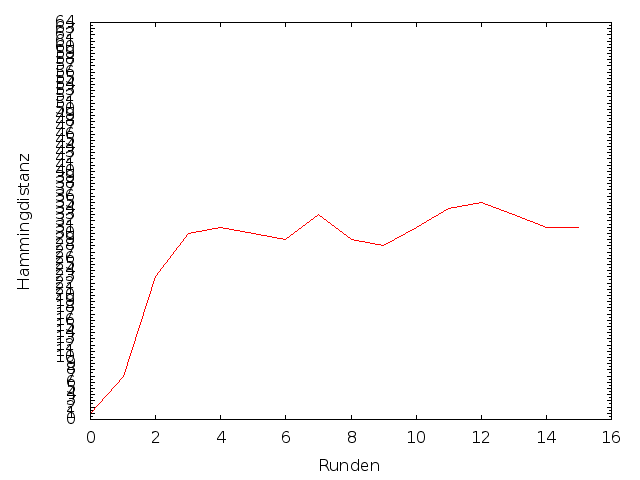
\includegraphics[scale=0.5]{ueb1_4.png}
\end{center}

\begin{table}[T]
\centering
\begin{tabular}{rr|rr}
Round $k$ & $HD(M_k,M_k)$ &  $HD(M_{1_k},M_{1_k})$ & $HD(M_{1_k},M_{1_k})$ \\ \hline
 0 &1 & 39 & 35 \\
 1 &7 &35 &31      \\
 2 &23 &32 &33     \\ 
 3 &30 &36 &35     \\
 4 &31 &37 &34     \\
 5 &30 &31 &34     \\
 6 &29 &26 &30     \\
 7 &33 &26 &26     \\
 8 &29 &29 &26     \\
 9 &28 &29 &34     \\
10 &31 &25 &36     \\
11 &34 &28 &35     \\
12 &35 &30 &38     \\
13 &33 &29 &37     \\
14 &31 &32 &38     \\
15 &31
\\ \hline								
\end{tabular}
\end{table}
\section{Übung 2}

\subsection{Aufgabe 1}

\subsubsection{Verschiebechiffren}

\begin{align}
	E_1: & z \mapsto (z +k_1)~\mod n \\
	E_2: & z \mapsto (z +k_2)~\mod n 
\end{align}

Dann wäre die Verkettung $ E_2 \circ E_1 $ :

\begin{align}
	E_2 \circ E_1 & = E_2(E_1(z)) =  (((z +k_1)~\mod n) +k_2)~\mod n \\
	              & = z+\underbrace{k_1+k_2}_{k_3} ~\mod n \\
	              & = z+k_3 ~\mod n = E_3(z)
\end{align}

Wir folgern daraus, dass eine Verkettung von zwei Verschiebechiffren keine zusätzlichen Gewinn bringt.

\subsubsection{Multiplikative Chiffren}

\begin{align}
	E_1: & z \mapsto (z \cdot  t_1)~\mod n \\
	E_2: & z \mapsto (z \cdot  t_2)~\mod n 
\end{align}

Dann wäre die Verkettung $ E_2 \circ E_1 $ :

\begin{align}
	E_2 \circ E_1 & = E_2(E_1(z)) =  (((z  \cdot t_1)~\mod n)  \cdot t_2)~\mod n \\
	              & = z \cdot \underbrace{t_1 \cdot t_2}_{t_3} ~\mod n \\
	              & = z \cdot t_3 ~\mod n = E_3(z)
\end{align}

Wir folgern daraus, dass eine Verkettung von zwei Multiplikativen Chiffren keine zusätzlichen Gewinn bringt.


\subsubsection{Tauschchiffren}

\begin{align}
	E_1: & z \mapsto (z \cdot t_1 + k_1)~\mod n \\
	E_2: & z \mapsto (z \cdot  t_2 + k_2)~\mod n 
\end{align}

Dann wäre die Verkettung $ E_2 \circ E_1 $ :

\begin{align}
	E_2 \circ E_1 & = E_2(E_1(z)) =  (((z  \cdot t_1 + k_1)~\mod n)  \cdot t_2 +k_2)~\mod n \\
	              & = z \cdot \underbrace{t_1 \cdot t_2}_{t_3} + \underbrace{k_1 \cdot t_2 + k_2}_{k_3} ~\mod n \\
	              & = z \cdot t_3 + k_3~\mod n = E_3(z)
\end{align}

Wir folgern daraus, dass eine Verkettung von zwei Tauschchiffren keine zusätzlichen Gewinn bringt.

\subsection{Aufgabe 2}

\subsubsection*{Berechnen Sie die multiplikativen Inverse zu $3,~5 ~\text{und} ~22~$ in $Z_23$.}

\begin{align*}
	23 & = 7 \cdot 3 + 2 \\
     3 & = 1 \cdot 2 + 1 \\
     2 & = 2 \cdot 1 + 0 
\end{align*}

\begin{align*}
	 1 & = 3 - 2 \\
     1 & = 3 - (23 - 7 \cdot 3 ) = \\
     1 & = \underline{8} \cdot - 1 \cdot 23    
\end{align*}


\begin{align*}
	23 & = 1 \cdot 15 + 8 \\
    15 & = 1 \cdot 8 + 7 \\
     8 & = 1 \cdot 7 + 1 \\     
     7 & = 7 \cdot 1 + 0     
\end{align*}

\begin{align*}
	 1 & = 8 - 7 \\
	 1 & = (23-15) - (15 - 8)        \\
	 1 & = (23-15) - (15 - (23-15))  \\
	 1 & = 23 - 15  - 15 + 23 - 15   \\
	 1 & = \underbrace{\underline{- 3}}_{20} \cdot 15 + 2 \cdot 23 	 	 
\end{align*}

\begin{align*}
	23 & = 1 \cdot 22 + 1 \\
    22 & = 22 \cdot 1 + 0 \\
\end{align*}

\begin{align*}
	 1 & = 1 \cdot 23 \underbrace{ \underline{- 1}}_{22} \cdot 22 \\
\end{align*}

\subsubsection*{Berechnen Sie die multiplikativen Inversen zu $3,~ 15 ~\text{und} ~22 ~\text{in}~ Z_{24}.$}

\begin{align*}
	24 & = 3 \cdot 8 + 0 \\
	&\Rightarrow \neg \exists ~ \text{multiplikatives Inverses}
\end{align*}

\begin{align*}
	24 & = 1 \cdot 15 + 9 \\
 	15 & = 1 \cdot 9 + 6 \\
	9 & = 1 \cdot 6 + 3 \\
	6 & = 2 \cdot 3 + 0 \\
	&\Rightarrow \neg \exists ~ \text{multiplikatives Inverses}
\end{align*}

\begin{align*}
	24 & = 1 \cdot 22 + 2 \\
 	22 & = 11 \cdot 2 + 0 \\
	&\Rightarrow \neg \exists ~ \text{multiplikatives Inverses}
\end{align*}

\subsubsection*{Zeigen Sie, dass $~(n-1)~$ in $Z_n$ bzgl. der Multiplikation zu sich selbst invers ist.}

\begin{align}
	(n-1) \cdot (n-1) & \equiv_n n^2 -2n + 1 \\
					  & \equiv_n 1 \mod ~ n
\end{align}



\subsection{Aufgabe 3}

Alphabet: \verb+ABCDEFGHIJKLMNOPQRSTUVWXYZ+
Alphabet: \verb+UEBRDNWOLKMSIFHTACGJPQVXYZ+

\begin{verse}
Wind Nord-Ost, Startbahn null-drei,\\
Bis hier hör ich die Motoren.\\
Wie ein Pfeil zieht sie vorbei,\\
Und es dröhnt in meinen Ohren.\\
Und der nasse Asphalt bebt,\\
Wie ein Schleier staubt der Regen,\\
Bis sie abhebt und sie schwebt\\
Der Sonne entgegen.\\
Über den Wolken\\
Muß die Freiheit wohl grenzenlos sein.\\
Alle Ängste, alle Sorgen, sagt man,\\
Blieben darunter verborgen und dann\\
Würde, was hier gross und wichtig erscheint,\\
Plötzlich nichtig und klein.\\
\end{verse}




\subsection{Aufgabe 4}

\subsubsection{}
Die Playfair-Verschlüsselung stellt eine Substitution für Buchstaben-Paare dar. 
Es handelt sich um eine bigraphische monoalphabetische Methode.
 Ähnlich wie bei der einfachen (monographischen) Buchstabensubstitution,
  beruhen Methoden zur Entzifferung von Playfair im Wesentlichen auf einer 
  Analyse der Häufigkeitsverteilung hier der Buchstabenpaare (Bigramme).
   In der deutschen Sprache beispielsweise sind die Bigramme "er", "en" und "ch" sehr häufig. Im Beispieltext fallen die "Doppler" (also Bigramm-Wiederholungen) ME…ME, IK…IK, QC…QC und TE…TE sowie die "Reversen" (Wiederholung eines umgedrehten Bigramms) CQ…QC auf, die sich in gleicher Weise im englischen Klartext wiederfinden.
Da kein Buchstabe mit sich selbst gepaart wird, gibt es nur 600 (25×24) mögliche Buchstabenkombinationen, 
die substituiert werden. Überdies gibt es eine Reihe von Symmetrien, die teilweise schon am obigen Beispieltext erkannt werden können.
So hilft der erwähnte Klartext-Geheimtext-Zusammenhang EL ↔ CQ und LE ↔ QC 
beim Bruch des Textes. Ist nämlich ein Bigramm geknackt, dann ist auch sofort das reverse (umgedrehte) Bigramm bekannt.
In den Fällen des Überkreuz-Schrittes gibt es darüber hinaus noch weitere Beziehungen zwischen den vier auftretenden Buchstaben
 in der Art (vgl. beispielsweise obere linke Ecke des Quadrats) DC ↔ EB, CD ↔ BE, EB ↔ DC sowie BE ↔ CD, die der Angreifer zur
  Entzifferung ausnutzen kann. Ferner hat auch die geschilderte Methode zur Erzeugung des Playfair-Quadrats Schwächen, denn
   es endet häufig – wie auch im Beispiel – auf "XYZ".
Die Playfair-Verschlüsselung ist somit weit entfernt von einer allgemeinen bigraphischen Methode
 mit völlig willkürlicher Zuordnung der Buchstabenpaare und stellt in der heutigen Zeit
  kein sicheres Verschlüsselungsverfahren mehr dar. So lassen sich mit modernen Mitteln
   auch relativ kurze Playfair-Texte in sehr kurzer Zeit brechen.


\subsection{Aufgabe 5}

Herleitung des Gleichungssystems: 

\begin{align}
H x_1+Ix_2 &= \ddot{A}  & Lx_1+Lx_2 = U \\
H x_3+Ix_4 &= U  & Lx_3+Lx_4 = K \\
\end{align}

\begin{math}
\begin{pmatrix}
7 & 8 & 0 & 0 \\ 
0 & 0 & 7 & 8 \\ 
11 & 11 & 0 & 0 \\ 
0 & 0 & 11 & 11
\end{pmatrix}
\begin{pmatrix} x_1 \\x_2 \\x_3 \\x_4 \end{pmatrix}
=
\begin{pmatrix} 26 \\ 20 \\ 20 \\ 10 \end{pmatrix}
\end{math}


\begin{align}
\begin{gmatrix}[p]
7 & 8 & 0 & 0   & 26 \\ 
0 & 0 & 7 & 8   & 20 \\ 
11 & 11 & 0 & 0 & 20 \\ 
0 & 0 & 11 & 11 & 10
\rowops
\swap{1}{2}
\end{gmatrix} &
\begin{gmatrix}[p]
7 & 8 & 0 & 0   & 26 \\ 
11 & 11 & 0 & 0 & 20 \\ 
0 & 0 & 7 & 8   & 20 \\ 
0 & 0 & 11 & 11 & 10
\rowops
\mult{0}{\cdot 7^{-1}  = 25 }
\mult{1}{\cdot 11^{-1} =  8 }
\mult{2}{\cdot 7^{-1}  = 25 }
\mult{3}{\cdot 7^{-1}  =  8 }
\end{gmatrix}\\[5mm]
\begin{gmatrix}[p]
1 & 26 & 0 & 0   & 12 \\ 
1 & 1 & 0 & 0 & 15 \\ 
0 & 0 & 1 & 26   & 7 \\ 
0 & 0 & 1 & 1 & 22
\rowops
\add[\cdot -1]{0}{1}
\add[\cdot -1]{2}{3}
\end{gmatrix}&
\begin{gmatrix}[p]
1 & 26 & 0 & 0   & 12 \\ 
0 & 4 & 0 & 0 & 3 \\ 
0 & 0 & 1 & 26   & 7 \\ 
0 & 0 & 0 & 4 & 22
\rowops
\mult{1}{\cdot 4^{-1}=22}
\mult{3}{\cdot 4^{-1}=22}
\end{gmatrix}\\[5mm]
\begin{gmatrix}[p]
1 & 26 & 0 & 0   & 12 \\ 
0 & 1 & 0 & 0 & 8 \\ 
0 & 0 & 1 & 26   & 7 \\ 
0 & 0 & 0 & 1 & 11
\rowops
\add[\cdot -26]{1}{0}
\add[\cdot -26]{3}{2}
\end{gmatrix}&
\begin{pmatrix} 7 \\  8 \\  11 \\  11\end{pmatrix}  =
\begin{pmatrix} H \\  I \\  L \\  L\end{pmatrix} 
\end{align}

\paragraph*{Bildung der Inversen $K^{-1}$}

\begin{align*}
\begin{gmatrix}[p]
 7 &  8 & 1 &0  \\
11 & 11 & 0 &1
\rowops 
\mult{0}{\cdot 7^{-1} = 25}
\end{gmatrix} &
\begin{gmatrix}[p]
 1 &  26 & 25 &0  \\
11 & 11 & 0 &1
\rowops 
\add[\cdot 11^{1}]{0}{1}
\end{gmatrix} \\
\begin{gmatrix}[p]
 1 &  26 & 25 &0  \\
 0 &  15 & 15 &1   
\rowops 
\mult{1}{\cdot 15^{-1} = 2}
\add[\cdot 26]{1}{0}
\end{gmatrix} &
\begin{gmatrix}[p]
1 & 0 & 28 & 6 \\
0 & 1 & 1 & 2
\end{gmatrix} 
\end{align*}

\begin{equation} K^{-1} = 
\begin{pmatrix}
28 & 6 \\ 
1 & 2
\end{pmatrix} 
\end{equation}

\textbf{Lösung: HILLISTEINFACHZUKNACKEN}

\subsection{Aufgabe 6}
\subsubsection{Warum gilt für zufällige Texte $I_r = \sfrac{1}{26} = 0.0385$?}

Wirklicher Zufall würde bedeuten das jeder Buchstaben $a \in A$ gleich oft im Text vorkommt.
Folglich handelt es sich um einen Laplace-Raum (wie beim Würfel) und die Warscheinlichkeit für $P(X = a) = \dfrac{1}{|A|}$.
In unseren Fall ist $ |A|=26 $.

%\begin{align}
%I = \dfrac{\sum_{i=1}{26} m_i (m_i-1)}{m(m-1)} }}
%m_1 = m_2 = m_3 = \cdots =  m_26 \\
%I = 0,0469
%\end{align}

\subsubsection{}
\subsubsection{}

\subsection{Übungsaufgabe: One-Time-Pad}

\begin{align}
P_1 &= hike = 001~ 010~ 011~ 000  \\
P_2 &= rike = 101~ 010~ 011~ 000  \\
C   &= eier = 000~ 010~ 000~ 101  \\
K   &= klet = 011~ 100~ 000~ 111  \\
\end{align}

\subsubsection{}

\begin{align}
 001~ 010~ 011~ 000 &\xor \\
 000~ 010~ 000~ 101 &=   \\
 001~ 000~ 011~ 101 &= hekr
\end{align}

\begin{align}
 101~ 010~ 011~ 000 &\xor \\
 000~ 010~ 000~ 101 &=   \\
 101~ 000~ 011~ 101 &= rekr
\end{align}

\subsubsection{}

\begin{align}
 001~ 010~ 011~ 000 &\xor \\
 011~ 100~ 000~ 111 &=   \\
 010~ 110~ 011~ 111 &= iskt
\end{align}

\begin{align}
 101~ 010~ 011~ 000~ &\xor \\
 011~ 100~ 000~ 111~ &=   \\
 110~ 110~ 011~ 010~ &= sski
\end{align}

\subsubsection{}

wenn $C_{1_i} = C_{2_i} \Rightarrow P_{1_i} = P_{2_i}$ 

\begin{equation}
C_1 \xor C_2 = (P_1 \xor K) \xor (P_2 \xor K) = P_1 \xor P_2 
\end{equation}

\subsubsection{}

\begin{align}
K &= C_1 \xor P_1 \\
C_2 \xor K &= P_2
\end{align}


\subsection{Skytale}
\subsubsection{}

\begin{align}
E(k, x_1 , \ldots , x_{km} ) &= \\
x_1 x_{m+1} x_{2m+1} \ldots x_{(k−1)m+1} x_{2} x_{m+2} x_{2m+2} \ldots x_{(k−1)m+2} \ldots x_m x_{2m} x_{3m} \ldots x_km
\\
\begin{pmatrix}
x_1 & x_2 & \cdots & x_m \\ 
x_{m+1} & x_{m+2} & \cdots & x_{2m} \\ 
\vdots & \vdots & \ddots & \vdots \\ 
x_{(k-1)m+1} & x_{(k-1)m+2} & \cdots & x_{km}
\end{pmatrix} 
\end{align}


%f(x) = K * x mod (N'-1)
%N' = K [N/K] für x \in N x startet bei 0
%f(x) = N/K xmod (N-1)

Ist die Klartextlänge kein Vielfaches von k, so kann der Klartext durch das Ein- bzw.
Anfügen von sogenannten Blendern (Füllzeichen) verlängert werden. Damit der Emp\-
fänger diese Füllzeichen nach der Entschlüsselung wieder entfernen kann, ist lediglich
darauf zu achten, dass sie im Klartext leicht als solche erkennbar sind.

\section{Moderne Symmetrische Chiffren}

\subsection{Lineare Abbildungen}


\subsection{Feistel-Cipher}
\subsubsection{}
$F: \{0, 1\}^4 \times \{0, 1\}^4 \to \{0, 1\}^4 $ mit $F(X, Y) = X \xor Y$\\
die Rundenzahl $n = 2$,\\
der Plaintext $ P = 10011100$ und\\
die Rundenschlüssel $K_1 = 0101 $und $K_2 = 1100$.
\paragraph{Berechnen Sie den Ciphertext $C$.}

\begin{align}
 L_i &= R_{i-1}\\
 R_i &= L_{i−1} \xor F(R_{i−1}, K_i)
\end{align}

\begin{tabular}{cc|ll}
Rnd & $K_i$ & $L_i$  & $R_i$    \\ \hline
0   & ---   & 1001 & 1100  \\
1   & 0101  & 1100 & 0000  \\
2   & 1100  & 0000 & 0000  
\end{tabular}

\paragraph{Berechnen Sie aus $C$ wieder den Plaintext $P$}.


\begin{align}
 R_{i} &= L_{i+1}  \\
 L_{i} &= R_{i+1} \xor F(R_{i},K_{i+1})
\end{align}

\begin{tabular}{cc|ll}
Rnd & $K_i$ & $L_i$  & $R_i$    \\ \hline
2   & 1100  & 0000 & 0000 \\
1   & 0101  & 1100 & 0000 \\
0   & ---   & 1001 & 1100  
\end{tabular}


\subsubsection{}
Eine Feistel-Funktion ist definiert durch $F(X, Y) = X$. Berechnen Sie den Ciphertext
$C$ in Abhängigkeit von einer beliebigen Rundenzahl $n$ und dem Plaintext $P = (L_0, R_0)$
Wie gut ist die dadurch erreichte Verschlüsselung?

\begin{tabular}{cc|>{$}c<{$}>{$}c<{$}}
Rnd & $K_i$ & L_i  & R_i    \\ \hline
0   & ---   & a        & b         \\
1   & ---   & b        & b \xor a  \\
2   & ---   & b \xor a & a         \\  
3   & ---   & a        & b         \\  
\end{tabular}

\begin{equation}
f(n, (a,b) ) = %
	\begin{cases}
	(a,b)        ,& n \mod 3 = 0 \\
	(b,b \xor a) ,& n \mod 3 = 1 \\
	(b \xor a,a) ,& n \mod 3 = 2 
	\end{cases}
\end{equation}


\subsection{DES-Details}
\subsubsection{Zeigen Sie, dass die DES-Expansionspermutation eine lineare Abbildung ist.}

\begin{equation}
A = \begin{array}{*{14}{r}}
(& 31 &  0 &  1 &  2 &  3 &  4 &  3 &  4 &  5 &  6 &  7 &  8 & \\
 &  7 &  8 &  9 & 10 & 11 & 12 & 11 & 12 & 13 & 14 & 15 & 16 & \\
 & 15 & 16 & 17 & 18 & 19 & 20 & 19 & 20 & 21 & 22 & 23 & 24 & \\
 & 23 & 24 & 25 & 26 & 27 & 28 & 27 & 28 & 29 & 30 & 31 &  0 &)
\end{array}
\qquad 
\end{equation}
Sei $P \in \mathbb{N}^{32 \times 48}$ die entsprechende Permutationsmatrix für $A$ 
und $f:\, A^{32} \to A^{48} ,\quad x \mapsto P \cdot x$ die Permutationsfunktion.

\textbf{zZ: f ist linear}\\

Sei $ x,y \in A^{32} $ mit $ x = (x_0, x_1, \ldots, x_{31} )$ und 
 $ y = (y_0, y_1, \ldots, y_{31} )$ 
 dann ist

\begin{align}
f(\alpha x) &=  \begin{array}{*{14}{r}}
(&\alpha x_{31} &  \alpha x_{0} &  \cdots &  \alpha x_{8} \\
 &\alpha x_{7}  &  \alpha x_{8} &  \cdots & \alpha x_{16} \\
 &\alpha x_{15} &  \alpha x_{16} & \ddots & \vdots        \\
 &\alpha x_{23} &  \alpha x_{24} & \cdots & \alpha x_{0}  &)\\
\end{array} \\
& = \alpha  \begin{array}{*{12}{r}}
 &(x_{31} &  x_{0} &  \cdots &  x_{8} \\
 & x_{7}  &   x_{8} &  \cdots &  x_{16} \\
 &x_{15} &   x_{16} & \ddots & \vdots        \\
 &x_{23} &   x_{24} & \cdots &  x_{0} &) \\
\end{array}\\
&= \alpha f(x)
\end{align}

\begin{align}
f(x+y) &=  \begin{array}{*{14}{r}}
(& x_{31} + y_{31} &  x_{0}  +y_{0}  &  \cdots &  x_{8} + y_{8}\\
 & x_{7}  + x_{7}  &  x_{8}  +y_{8}  &  \cdots & x_{16} + y_{16} \\
 & x_{15} + y_{15} &  x_{16} +y_{16} &  \ddots & \vdots        \\
 & x_{23} + y_{23} &  x_{24} +y_{24} &  \cdots & x_{0} +y_{0} &)
\end{array} \\
 & = \begin{array}{*{12}{r}}
 &(x_{31} &  x_{0} &  \cdots &  x_{8} \\
 & x_{7}  &   x_{8} &  \cdots &  x_{16} \\
 &x_{15} &   x_{16} & \ddots & \vdots        \\
 &x_{23} &   x_{24} & \cdots &  x_{0} &) \\
\end{array} + 
\begin{array}{*{12}{r}}
 &(y_{31} &  y_{0} &  \cdots & y_{8} \\
 & y_{7}  &   y_{8} &  \cdots &  y_{16} \\
 &y_{15} &   y_{16} & \ddots & \vdots        \\
 &y_{23} &   y_{24} & \cdots &  y_{0} &) \\
\end{array}\\
&= f(x)+f(y)
\end{align}
\qed

\subsubsection{Zeigen Sie, dass die DES S-Boxen keine lineare Abbildung sind.}

\textbf{zZ. $S_i$ ist nicht linear.} 
Wir nehmen die S1-Box und sei $x = 0 \wedge \alpha = 2$ 

\begin{align}
 \operatorname*{S1}(\alpha x) &=  \operatorname*{S1}(000000_2)      \\
				              &= 1110_2  = 14_{10}                  
\end{align}
\begin{align}
  \alpha  \operatorname*{S1}(x) &= 2 \operatorname*{S1}(000000_2)  \\
				 &= 2_{10} * 1110_2 = 28_{10}
\end{align}
\begin{equation}
\Rightarrow 	\operatorname*{S1}(\alpha x) \ne \alpha \operatorname*{S1}(x)			
\end{equation}
\qed

\subsubsection{Geben Sie für die DES-Permutation die Zykelschreibweise an.}
\begin{equation}
A = \left (\begin{array}{*{32}{r}}
0&1&2&3&4&5&6&7&8&9&10&11&12&13&14&15&16&17&18&19&20&21&22&23&24&25&26&27&28&29&30&31	\\
15&6&19&20&28&11&27&16&0&14&22&25&4&17&30&9&1&7&23&13&31&26&2&8&18&12&29&5&21&10&3&24
\end{array}\right )
\end{equation}
	
\begin{equation}
\text{Zyklen:}  
(0\,15\,9\,14\,30\,3\,20\,31\,24\,18\,23\,8)
(1\,6\,27\,5\,11\,25\,12\,4\,28\,21\,26\,29\,10\,22\,2\,19\,13\,17\,7\,16)
\end{equation}												

\subsubsection{Zeigen Sie, dass für den DES Schlüssel $K = 0xE0E0E0E0F1F1F1F1$
(inklusive Parity-Bits) alle Rundenschlüssel identisch sind. Warum gilt in
diesem Fall $DES(K, DES(K, M)) = M$ (d.h. Ver- und Entschlüsselung sind
identisch)?}

\begin{equation}
K=\begin{matrix}
1 & 1 & 1 & 0 & 0 & 0 & 0 & 0 \\
1 & 1 & 1 & 0 & 0 & 0 & 0 & 0 \\
1 & 1 & 1 & 0 & 0 & 0 & 0 & 0 \\
1 & 1 & 1 & 0 & 0 & 0 & 0 & 0 \\
1 & 1 & 1 & 1 & 0 & 0 & 0 & 1 \\
1 & 1 & 1 & 1 & 0 & 0 & 0 & 1 \\
1 & 1 & 1 & 1 & 0 & 0 & 0 & 1 \\
1 & 1 & 1 & 1 & 0 & 0 & 0 & 1 
\end{matrix} \xrightarrow{PC1}
\begin{matrix}
1 & 1 & 1 & 1 & 1 & 1 & 1 \\
1 & 1 & 1 & 1 & 1 & 1 & 1 \\
1 & 1 & 1 & 1 & 1 & 1 & 1 \\ 
1 & 1 & 1 & 1 & 1 & 1 & 1 \\ 
0 & 0 & 0 & 0 & 0 & 0 & 0 \\ 
0 & 0 & 0 & 0 & 0 & 0 & 0 \\ 
0 & 0 & 0 & 0 & 0 & 0 & 0 \\ 
0 & 0 & 0 & 0 & 0 & 0 & 0 
\end{matrix}
\end{equation}

Da alle in den folgenden Runden lediglich zu Spaltentransposition kommt und jede Spalte gleich sind, 
sind alle $C_i,D_i$ für alle $1 \le i \le 16$.


\subsection{A5/1}

\begin{align}
X = (x_0, x_1 \cdots , x_{18}) &= (1010101010101010101)    \\
Y = (y_0, y_1, \cdots , y_{21}) &= (1100110011001100110011) \\
Z = (z_0, z_1, \cdots , z_{22}) &= (11100001111000011110000)
\end{align}

\begin{algorithm}[H]
%Initialisiere X,Y,Z\;
\While{True}{
  $m = maj(x_8, y_{10}, z_{10})$\;
  \If{$x_8 = m$}{
    $t = x13 \xor x16 \xor x17 \xor x18$\;
    shift $t$ into $X$\;
  }	
  \If{$y_{10} = m$}{
    $t = y_{20} \xor y_{21} $\;
    shift $t$ into $Y$\;
  }
  \If{$z_{10} = m$}{
    $t = z_7 \xor z_{20} \xor z_{21} \xor z_{22}$\;
    shift $t$ into $Y$\;
  }
  $k_i = x_{18} \xor y_{21} \xor z_{22}$\;	
}
\end{algorithm}

\subsubsection{}
\scalebox{0.85}{
\begin{tabular}{*{4}{l}|c*{3}{l}|c}
Rnd & $x_8$ & $y_{10}$  & $z_{10}$ & m &  $X'$ & $Y'$ & $Z'$ & Bit \\ \hline  
 1  & 1
    & 0
    & 1
    & 1 
    & \ttfamily \textbf{0}101010101010101010\textit{1}  
    & \ttfamily 1100110011001100110011
    & \ttfamily \textbf{0}1110000111100001111000\textit{0} 
    & 1 \\ \hline
    
 2  & 0
    & 0
    & 1
    & 0 
    & \ttfamily \textbf{0}010101010101010101\textit{0}
    & \ttfamily \textbf{0}110011001100110011001\textit{1}
    & \ttfamily 01110000111100001111000
    & 0 \\ \hline   
    
 3  & 1
    & 1
    & 1
    & 1 
    & \ttfamily \textbf{1}001010101010101010\textit{1}
    & \ttfamily \textbf{0}011001100110011001100\textit{1}
    & \ttfamily \textbf{1}0111000011110000111100\textit{0}
    & 0 \\ \hline         
\end{tabular}}

\subsubsection{}
\lstset{language=Java}
\lstinputlisting{src/A51.java}
 
\subsection{RC4}

\lstset{language=Java}
\lstinputlisting{src/RC4.java}
\section{Hashfunktionen und MACs}
\subsection{Funktionsweise von Hash-Funktionen}

\begin{eqnarray}
	 Y                      & = 11110 \\
	 F:                     & \{0,1\}^4 \rightarrow \{0,1\}^2 ,\\
	 (x_1, x_2, x_3, x_4) & \mapsto (x_1 \xor x_4, x_2 \xor x_3)
\end{eqnarray}

\begin{center}
\begin{tabular}{cc|cc|c}
$x_1$ & $x_2$ & $x_3$ & $x_4$ & $F(x_1,x_2,x_3,x_4)$ \\
$0$ & $0$ & $1$ & $1$ & $11$ \\
$1$ & $1$ & $1$ & $1$ & $00$ \\
$0$ & $0$ & $0$ & $0$ & $00$ \\
\end{tabular}
\end{center}

\subsection{Kollisionen und Preimage-Angriffe}
\[ X = (X_0,X_1,X_2, \ldots , X_{n-1}) \]
\[H(X) = nX_0 + (n - 1)X_1 + (n - 2)X_2 + \ldots +2X_{n−2} + X_{n−1} \mod 256 = \sum\limits_{i\ge 0}^n (n-i)X_i \mod 256 \]
\subsubsection{Berechnen Sie H(X) für die Nachricht "FHT4ever". Interpretieren Sie dabei jeden Buchstaben als seinen 8 Bit ASCII-Wert.}
\begin{align}
X    &= (70, 72, 84, 52, 101, 118, 101, 114) \\
H(X) &= 8 \cdot 70 + 7 \cdot 72 + 6 \cdot 84 + 5 \cdot 52 + 4 \cdot 101 + 3 \cdot 118 + 2 \cdot 101 + 114\\
     &= 560 + 504 + 504 + 260 + 404 + 354 + 202 + 114 \\
     &= 48 + 248 + 248 + 4 + 148 + 98 + 202 + 114     \\
     &= 86
\end{align}

\begin{lstlisting}
H = lambda x: sum([(len(x)-i)*ord(e)\%256 for i,e in enumerate(x)])\%256
\end{lstlisting}

\subsubsection{Finden Sie eine andere (sinnvolle) Nachricht, die den gleichen Hashwert wie "FHT4ever" hat.}

\[  H(Uni4ever) = 86 \]

\subsubsection{Gegeben sei $h(X)=42$, wobei $X = (X_0,X_1,X_2)$. Finden Sie ein $Y =(Y_0,Y_1,Y_2)$ mit $X ≠ Y \wedge
h(Y) = h(X)$.}
\subsubsection{Finden Sie eine weitere Kollision.}


\begin{align}
	H(X) = 42 &= (3 X_1 + 2 X_2 + X_1) \mod 256 	        
\end{align}


Folgende Tabelle gibt Tupeln   $X = (X_0,X_1,X_2)$ mit  $H(X) = 42$ an. 
Insgesamt existieren 65536 Kollision (ExhaustedSearch).
\begin{lstlisting}
	c = [ (x,y,z) for x in range(256) 
                    for y in range(256) 
                      for z in range(256)
                        if (3*x+2*y+z) % 256==42 ]
	print len(c)
\end{lstlisting}
\begin{center}
\begin{tabular}{ccc}
$X_1$&$X_2$&$X_3$\\
96 & 166 & 190 \\
96 & 167 & 188 \\
96 & 168 & 186 
\end{tabular}
\end{center}



\subsection{Das Online-Auktionshaus}

\subsubsection{Denken Sie sich ein möglichst einfaches Verfahren aus, das auf einer Hash-Funktion beruht.}

Ein Gebot ist ein Hashwert bestehend aus: Betrage, Timestamp und Nonce $$H(( bid \circ time \circ salt) ) = Y$$
Die anderen Bieter können nicht errechnen welchen Betrag ein Bieter geboten hat,
da die Umkehrung von $H$ nicht möglich ist.

Sobald die Bieterrunde geschlossen wird, schickt jeder Bieter sein Gebot, Timestamp und Nonce zum Auktionator. 
Dieser kann nun die Hashwerte der Gebote überprüfen und den günstigen Bieter ermitteln.

Folgendes Bild zeigt ein Beispielablauf einer Auktion.

\begin{center}
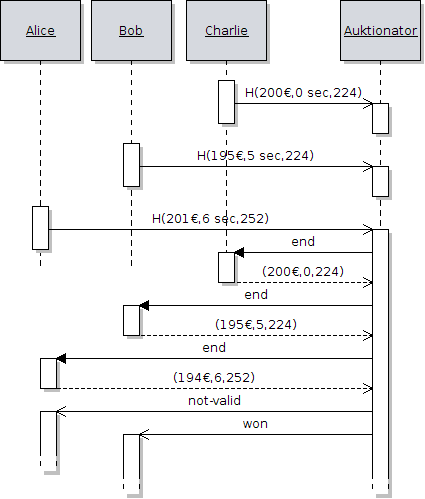
\includegraphics[scale=0.5]{images/auction-bidding.png}
\end{center}

Im Beispiel sehen, dass Alices Gebot abgelehnt wird da $$H(  201 \circ \ldots  ) = H( 196 \circ \ldots)$$
Sowie das Bob gewinnt, da er das günstigste Gebot abgeben hat.

\subsubsection{Welche Angriffe gibt es trotzdem noch auf das Verfahren?}

\begin{itemize}
\item Man-in-the-Middle Attake aufgrund fehlender Authentizität.
\item Störungen des Übertragungskanals
\item ohne Timetamp wäre Replayangriffe möglich
\item ohne Salt wäre die Authentifizierung komplett ausgehebelt
\end{itemize}

\subsection{Datenbankschutz durch Verschlüsselung und Hash-Funktionen}

\lstset{language=SQL}
\lstinputlisting{eclipse/member.db.sql}



\subsection{kryptologische Absicherung der Prüfungsvorleistung}
\subsubsection{Das Verfahren ist bisher kryptologisch nicht gesichert. Welche Angriffe sind denkbar?}
\begin{itemize}
\item Identitätsdiebstahl, man verwendet den Zettel eines anderen
\item Replikation des eigenen Scheines mit Fälschung des Ergebnisses
\item Replikation eines anderen Scheines Fälschung der persönlichen Angaben
\end{itemize}

\subsubsection{Sichern Sie das Verfahren kryptologisch ab. 
               Der Professor soll die "Echtheit" der Bescheinigung möglichst einfach prüfen können.}
               
(1) Auf dem Schein wird ein QR-Code abgedruckt der einen Hash mit den Angaben auf dem Schein und einen geheimen Saltwert beinhaltet. Dies kann mit einem Handy leicht geprüft. Überprüfung der Identität ist weiterhin erforderlich.

(2) Verfahren (1) kann auch als Hex-Zeichen aufgedruckt werden.

(3) $H(Matrikel,Bestanden,Salt) = (Matrikel+Bestanden+Salt \mod N)$
\section{Übungsaufgaben: Asymmetrische Kryptologie}
\subsection{Rucksack}


PrivateKey: $(3,5,10,23), m= 8	, n = 47$

\subsubsection{Geben sie den öffentlichen Schlüssel an}

\begin{align}
	 3 \cdot 8 \mod 47 &= 24 \\
  	 5 \cdot 8 \mod 47 &= 40 \\
	10 \cdot 8 \mod 47 &= 33 \\
	23 \cdot 8 \mod 47 &= 43 	
\end{align}

PublicKey: $(24,40,33,43)$

\subsubsection{Verschlüsseln Sie $P=[1110 0000 0010]_2$ (Binärdarstellung) im ECB-Modus.}


\begin{align}
	C_1 = 1 \cdot 24 + 1  \cdot  40 + 1 \cdot 33 +0  \cdot 43 &= 97 \\ 
	C_2 = 0 \cdot 24 + 0  \cdot  40 + 0 \cdot 33 +0  \cdot 43 &= 0   \\ 	
	C_3 = 0 \cdot 24 + 0  \cdot  40 + 0 \cdot 33 +0  \cdot 43 &= 33 
\end{align}


\subsubsection{Finden Sie den Plaintext zum Ciphertext $C = (67, 64)$}

$ m^{-1} = 6 $:

$ C_1= 67 * 6 \mod 47 = 26 $

\begin{tabular}{ccc}
 $S_i$ & $ Cm^{-1} $ & $P$ \\ \hline
 23    & 26          & 1  \\
 10    & 3           & 0  \\
 5     & 3           & 0  \\
 3     & 0           & 1  \\
\end{tabular}


$P_1 = 1001$

$C_2= 64 * 6 \mod 47 = 8$


\begin{tabular}{ccc}
 $S_i$ & $Cm^{-1}$ & $P$ \\ \hline
 23    & 8  & 0  \\
 10    & 8  & 0  \\
 5     & 3  & 1  \\
 3     & 0   & 1  
\end{tabular}

$P_2 = 0011$

\subsection{RSA auf Nachricht in Blöcken}
\begin{align}
  P &= \text{'FHT4EVER'}  &  n &= 13 \cdot 17 = 221 & e &= 3
\end{align}


\textbf{Beachten: $ggT(e, \phi(221) ) \ne 1$}. Entschlüsselung damit ummöligch.

\begin{align}
	E(x) &=  x^3 \mod 221 \\
	E(P) &=  E('F') \circ E('H')\circ E('T')\circ E('4')\circ E('E')\circ E('V')\circ E('E')\circ E('R')\\
		 &=  \operatorname{apply}(x^3 \mod 221 ,[70, 72, 84, 52, 69, 86, 69, 82])    \\
		 &=  [8, 200, 203, 52, 103, 18, 103, 194]
\end{align}



\subsection{Chinesischer Restsatz}
\subsubsection{Es sei $m = 11, n = 12, a = 3$ und $b = 4$. Geben Sie ein $x$ an, für das gilt: $x \mod m = a$ und $ x \mod n = b$}

\begin{equation}
	x = a n N + b m M  = 3 \cdot 12 \cdot N + 4 \cdot 11 M
\end{equation}

\[ggT(12, 11) = 1 \text{ mit } a^{-1} = -1 = N\]
\[ggT(11, 12) = 1 \text{ mit } a^{-1} =  1 = M\]

\begin{align}
	X &= 3 \cdot 12 \cdot 1 + 4 \cdot 11 \cdot -1 \\
	  &=  36 - 44 = -8
\end{align}
\textbf{Probe:}
\begin{align}
	-8 \mod  m &= a  & -8 \mod  n &= b \\
	-8 \mod 11 &= 3  & -8 \mod 12 &= 4 \\
\end{align}

\subsubsection{Es sei $m = 11, n = 12, l = 12, a = 3, b = 4 \text{ und } c=5$. Geben Sie ein $x$ an, für das
gilt: $x \mod m = a$ und $x \mod n = b$ und $x \mod l = c$.}



\begin{align}
 X = a \cdot n \cdot l (nl)^{-1}
   + b \cdot m \cdot l (ml)^{-1}
   + c \cdot n \cdot m (nm)^{-1} \\
 x \mod 11 = 3 \\
  x \mod 12 &= 4\\
   x \mod 11 &= 5\\
\end{align}




\textbf{Vorrausetzung für Chin. Restsatz nicht erfüllt.}
$ggT(n,l)=12$ damit nicht relativ prim.


\subsubsection{Verallgemeinern Sie den Chinesischer Restsatz:
Gesucht ist $x$ mit $(x \mod m_i)=x_i$ und die passende Berechnungsvorschrift. Wie groß ist die Laufzeit zur Berechnung von x?}

\textbf{Eingabe}: $m_i$ die Module (paarweise relativ prim), $x_i$ die gesuchten Ergebnisse mit $1 \le i \le n$. 

Sei $N_j$ das Produkt von $ \prod_{i>0 \wedge i \ne j}^{n} m_i = 
	m_1 \cdots m_{j-1} \cdot m_{j+1} \cdots m_n$	
Sei $M_i$ multiplikative Inverse von $N_i$ zu $m_i$.

\begin{align}
	X &= \sum_{i}^{n} x_i \underbrace{N_i M_i}_{\equiv_{m_i} 1} \\
	  &= x_1 m_2 \cdots m_n M_1 + \ldots + x_n m_1 \cdots m_{n-1} M_n	
\end{align}

Kosten: $T = n \cdot T_{\text{egcd}} + n (n+1) T_{\text{mult}} + n T_{\text{add}} \in \mathcal{O}(n^2)$.

\subsection{RSA-Low-Exponent-Attack}
\subsubsection{Gg. seien die drei öffentlichen RSA-Schlüssel $(n_1 = 35,e=3)$,$(n_1 = 35,e=3)$,$(n_1 = 35,e=3)$.
Außerdem bekannt ist: $C_{123}=(22,12,216)$}

Voraussetzungen: 
	$$ C_{123} = P^3 \mod n_{123} $$
und $n_{123}$ sind paarweise relativ prim.

Gesucht $x$:
$$ x \mod n_{1} = C_{1} \wedge
   x \mod n_{2} = C_{2} \wedge
   x \mod n_{3} = C_{3} \wedge   $$



\begin{align}
	x = \underbrace{C_{1} n_{2} n_{3} N_{23}}_{\equiv 1 \mod n_1}
	  + \underbrace{C_{1} n_{1} n_{3} N_{13}}_{\equiv 1 \mod n_2}
	  + \underbrace{C_{1} n_{1} n_{2} N_{12}}_{\equiv 1 \mod n_3}
\end{align}

Suche der multiplikativen Inversen $N_{123}$ zum Modul $n_{123}$ mit erweiterter euklidischer Algorithmus:

$ggT(n_{2}n_{3},n_{1}) = ggT(24,35):$
\begin{align}
35 &= 1 \cdot 24+11			\\
24 &= 2 \cdot 11+2			\\
11 &= 5 \cdot 2+1			
\end{align}

\begin{align}
1 &= 11 - 5 \cdot 2						\\
1 &= 35 -24 - 5 \cdot (24-2 \cdot 11)	\\
1 &= -24 -5 \cdot (24-2 \cdot (35-24))  \\
1 &= -24 -5 \cdot (24+2 \cdot 24)		\\
1 &= -16 \cdot 24						\\
1 &=  19 \cdot 24						
\end{align}

$$N_{23} = 19$$

$ggT(n_{1}n_{3}, n_{2}) = ggT(8,143):$
\begin{align}
134   &= 17 \cdot 8+7			\\
8     &= 7+1
\end{align}

\begin{align}
1 = 8 -7						\\
1 = 8 -(143-17 \cdot 8)			\\
1 = 8+17 \cdot 8				\\
1 = 18 \cdot 8					
\end{align}

$$N_{13} = 18$$

$ggT(n_{1}n_{2}, n_{3}) = ggT(160,323):$
\begin{align}
323 = 2 \cdot 160+3\\
160 = 53 \cdot 3+1\\
\end{align}
\begin{align}
1 = 160-53 \cdot 3 \\
1 = 160-53 \cdot (323-2 \cdot 160) \\
1 = 107 \cdot 160
\end{align}

$$N_{12}= 107$$
	
\begin{equation}
	x = P^3 = 137.424.442 = 12.167 (mod n_{1}n_{2}n_{3})
\end{equation}
\begin{equation}
P=  \sqrt[3]{x} = \sqrt[3]{12167} = 23
\end{equation}

\textbf{Probe:}
\begin{equation}
23^3 \mod n_{123} = C_{123}
\end{equation}




\subsubsection{}

\subsection{Quadratwurzeln mod n}
				\[ 16 \mod 35 \]				
\subsubsection{mit chin. Restsatz}

Zerlegung in $pq=n$ mit $7 \cdot 5 = 35$.

Lösung von $16  \equiv 2 \mod 7$ mit Folgerung (2.5).

\[ 2^{\dfrac{7+1}{4}}  \imp x_1 = 4 \wedge x_2 = 7 - 4 = 3 \]

\noindent
Lösung von $16 \equiv 1 \mod 5$:

\[ x_3 = 1 \text{ und } x_4 = 4 \]

\begin{align}
	x & = 1 \mod 5 \label{eq:bbb}\\
	x & = 3 \mod 7 \label{eq:bba}\\ 
	x & = 4 \mod 7 \label{eq:bbc}\\
	x & = 4 \mod 5 
\end{align}


Betrachtung für  \eqref{eq:bbb} mit  \eqref{eq:bba} und \eqref{eq:bbc}  reicht:

\begin{equation}
	X = x_1 p P + x_2 q Q = 1 \cdot 7 P + 3 \cdot 5 Q
\end{equation}

$ggT(7,5)=1 a^{-1} = 3$
$ggT(5,7)=1 a^{-1} = 10$

\[	X_1 = 4\]


\begin{equation}
	X = x_3 p P + x_3 q Q = 4 \cdot 7 P + 4 \cdot 5 Q
\end{equation}

$ggT(7,5)=1 a^{-1} = 3$
$ggT(5,7)=1 a^{-1} = 10$

\[	X_2 = 9\]

Weitere \[X_3 = 35-X_1 = 31 \text{ und } X_4 = 35-X_2 \]

\subsubsection{}
[0, 1, 4, 9, 16, 25, 1, 14, 29, 11, 30, 16, 4, 29, 21, 15, 11, 9, 9, 11, 15, 21, 29, 4, 16, 30, 11, 29, 14, 1, 25, 16, 9, 4, 1]

\subsection{Rabin}

Sei der öffentliche Schlüssel $n=77$, der geheime Schlüssel $p=7$ und $q=11$.
Gegeben sei der Ciphertext $C = 23$.


\subsubsection{Wie lauten die möglichen Klartexte?}

Lösung für $x^2 \equiv_p C$ (2.5):    

\begin{equation}
	C^{\dfrac{7+1}{4}} \equiv_7  4
\end{equation}

\[ x_{12} = 4,3 \]

\noindent
Lösung für $x^2 \equiv_q C$ (2.5):    

\begin{equation}
	C^{\dfrac{11+1}{4}} \equiv_11  1
\end{equation}



\[ x_{34} = 1,10 \]

Mit dem Restsatz: \[X = (32,45,10,67)\]

\subsubsection{Sie wissen, dass der Klartext in seiner 7-Bit-Binärdaretsllung im höchsten Bit
eine "1" hat. Welches ist der gesuchte Klartext?}

$P=67$

\subsection{Elgamal}
Öffentlicher Schlüssel: $p = 2579$, Primitivwurzel $g = 2, y = 2765 = 949 \mod 2579$ \\
Geheimer Schlüssel: $x = 765$ \\
Nachricht: $m = 1299, k = 853$\\
\subsubsection{Führen Sie die Verschlüsselung durch.}

\begin{align}
	a&= g^k \mod p = 2^{853} \mod 2579 = 435 \\
	b&= y^km \mod p = 949^{853} \cdot 1299 \mod 2579 =2396
\end{align}

\[ C= (435,2396) \]

\subsubsection{Führen Sie die Entschlüsselung des Ciphertexts durch und überprüfen Sie, ob
Sie wieder m erhalten.}

\begin{align}
	P &= \dfrac{b}{a^x} \mod 2579= 
      &= \dfrac{2396}{436^{765}} \mod p  
	  &= \dfrac{2396}{2424} \mod p 
	  &= 2396 * 2424^{-1} \mod p
      &= 1299
\end{align}



\subsection{Diskrete Exponential-Funktion}

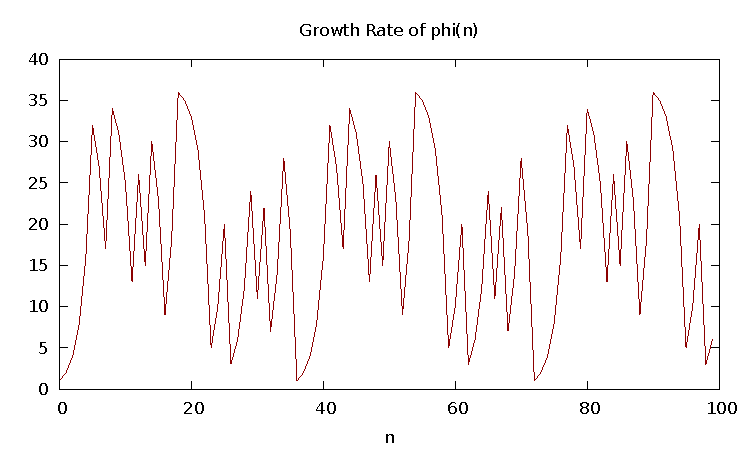
\includegraphics[scale=1]{eclipse/expofun.pdf}


\subsection{Primfaktorzerlegung}
\subsection{Fermatscher Primzahltest}

\subsection{Inverses zu $(n-1) \mod n$}
\subsection{$a(n-1) \mod n$}
\subsection{$\phi(n)$ für $n < 500$}
\subsubsection{Berechnen Sie $\phi(n)$ für $n < 500$ und tragen Sie die Werte in einem Graphen}

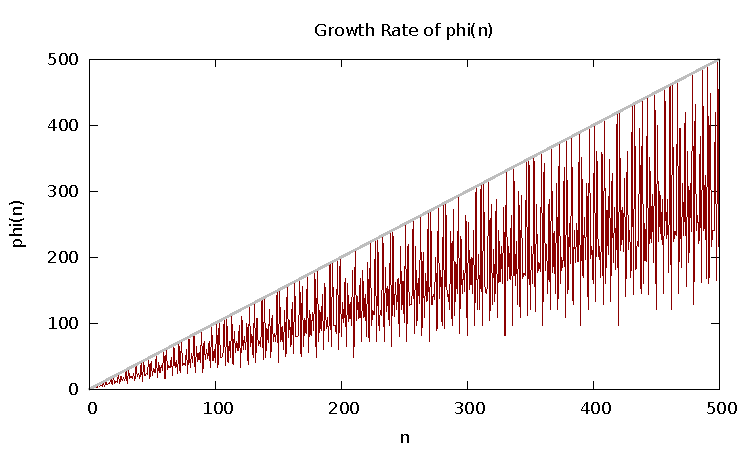
\includegraphics[scale=1]{eclipse/growth-rate.pdf}

\subsubsection{Geben Sie eine möglichst genaue obere Schranke für $\phi(n)$ an.}

\begin{align}
	 \phi(n) &\le n-1 \\
	         & \in \mathcal{O}(n)
\end{align}	


\end{document}


